
%% bare_conf.tex
%% V1.4b
%% 2015/08/26
%% by Michael Shell
%% See:
%% http://www.michaelshell.org/
%% for current contact information.
%%
%% This is a skeleton file demonstrating the use of IEEEtran.cls
%% (requires IEEEtran.cls version 1.8b or later) with an IEEE
%% conference paper.
%%
%% Support sites:
%% http://www.michaelshell.org/tex/ieeetran/
%% http://www.ctan.org/pkg/ieeetran
%% and
%% http://www.ieee.org/

%%*************************************************************************
%% Legal Notice:
%% This code is offered as-is without any warranty either expressed or
%% implied; without even the implied warranty of MERCHANTABILITY or
%% FITNESS FOR A PARTICULAR PURPOSE!
%% User assumes all risk.
%% In no event shall the IEEE or any contributor to this code be liable for
%% any damages or losses, including, but not limited to, incidental,
%% consequential, or any other damages, resulting from the use or misuse
%% of any information contained here.
%%
%% All comments are the opinions of their respective authors and are not
%% necessarily endorsed by the IEEE.
%%
%% This work is distributed under the LaTeX Project Public License (LPPL)
%% ( http://www.latex-project.org/ ) version 1.3, and may be freely used,
%% distributed and modified. A copy of the LPPL, version 1.3, is included
%% in the base LaTeX documentation of all distributions of LaTeX released
%% 2003/12/01 or later.
%% Retain all contribution notices and credits.
%% ** Modified files should be clearly indicated as such, including  **
%% ** renaming them and changing author support contact information. **
%%*************************************************************************


% *** Authors should verify (and, if needed, correct) their LaTeX system  ***
% *** with the testflow diagnostic prior to trusting their LaTeX platform ***
% *** with production work. The IEEE's font choices and paper sizes can   ***
% *** trigger bugs that do not appear when using other class files.       ***                          ***
% The testflow support page is at:
% http://www.michaelshell.org/tex/testflow/



\documentclass[conference]{IEEEtran}
% Some Computer Society conferences also require the compsoc mode option,
% but others use the standard conference format.
%
% If IEEEtran.cls has not been installed into the LaTeX system files,
% manually specify the path to it like:
% \documentclass[conference]{../sty/IEEEtran}





% Some very useful LaTeX packages include:
% (uncomment the ones you want to load)


% *** MISC UTILITY PACKAGES ***
%
%\usepackage{ifpdf}
% Heiko Oberdiek's ifpdf.sty is very useful if you need conditional
% compilation based on whether the output is pdf or dvi.
% usage:
% \ifpdf
%   % pdf code
% \else
%   % dvi code
% \fi
% The latest version of ifpdf.sty can be obtained from:
% http://www.ctan.org/pkg/ifpdf
% Also, note that IEEEtran.cls V1.7 and later provides a builtin
% \ifCLASSINFOpdf conditional that works the same way.
% When switching from latex to pdflatex and vice-versa, the compiler may
% have to be run twice to clear warning/error messages.






% *** CITATION PACKAGES ***
%
%\usepackage{cite}
% cite.sty was written by Donald Arseneau
% V1.6 and later of IEEEtran pre-defines the format of the cite.sty package
% \cite{} output to follow that of the IEEE. Loading the cite package will
% result in citation numbers being automatically sorted and properly
% "compressed/ranged". e.g., [1], [9], [2], [7], [5], [6] without using
% cite.sty will become [1], [2], [5]--[7], [9] using cite.sty. cite.sty's
% \cite will automatically add leading space, if needed. Use cite.sty's
% noadjust option (cite.sty V3.8 and later) if you want to turn this off
% such as if a citation ever needs to be enclosed in parenthesis.
% cite.sty is already installed on most LaTeX systems. Be sure and use
% version 5.0 (2009-03-20) and later if using hyperref.sty.
% The latest version can be obtained at:
% http://www.ctan.org/pkg/cite
% The documentation is contained in the cite.sty file itself.

\usepackage[pdftex]{graphicx}
\usepackage{smartdiagram}
\usesmartdiagramlibrary{additions}
\usepackage{cleveref}
\usepackage{booktabs} % Allows the use of \toprule, \midrule and \bottomrule in table
\usepackage{xspace,upgreek}
\usepackage{units_definitions}
\usepackage{tikz}
\usepackage{subfig}

% *** MATH PACKAGES ***
%
\usepackage{amsmath}
% A popular package from the American Mathematical Society that provides
% many useful and powerful commands for dealing with mathematics.
%
% Note that the amsmath package sets \interdisplaylinepenalty to 10000
% thus preventing page breaks from occurring within multiline equations. Use:
%\interdisplaylinepenalty=2500
% after loading amsmath to restore such page breaks as IEEEtran.cls normally
% does. amsmath.sty is already installed on most LaTeX systems. The latest
% version and documentation can be obtained at:
% http://www.ctan.org/pkg/amsmath





% *** SPECIALIZED LIST PACKAGES ***
%
%\usepackage{algorithmic}
% algorithmic.sty was written by Peter Williams and Rogerio Brito.
% This package provides an algorithmic environment fo describing algorithms.
% You can use the algorithmic environment in-text or within a figure
% environment to provide for a floating algorithm. Do NOT use the algorithm
% floating environment provided by algorithm.sty (by the same authors) or
% algorithm2e.sty (by Christophe Fiorio) as the IEEE does not use dedicated
% algorithm float types and packages that provide these will not provide
% correct IEEE style captions. The latest version and documentation of
% algorithmic.sty can be obtained at:
% http://www.ctan.org/pkg/algorithms
% Also of interest may be the (relatively newer and more customizable)
% algorithmicx.sty package by Szasz Janos:
% http://www.ctan.org/pkg/algorithmicx




% *** ALIGNMENT PACKAGES ***
%
%\usepackage{array}
% Frank Mittelbach's and David Carlisle's array.sty patches and improves
% the standard LaTeX2e array and tabular environments to provide better
% appearance and additional user controls. As the default LaTeX2e table
% generation code is lacking to the point of almost being broken with
% respect to the quality of the end results, all users are strongly
% advised to use an enhanced (at the very least that provided by array.sty)
% set of table tools. array.sty is already installed on most systems. The
% latest version and documentation can be obtained at:
% http://www.ctan.org/pkg/array


% IEEEtran contains the IEEEeqnarray family of commands that can be used to
% generate multiline equations as well as matrices, tables, etc., of high
% quality.




% *** SUBFIGURE PACKAGES ***
%\ifCLASSOPTIONcompsoc
%  \usepackage[caption=false,font=normalsize,labelfont=sf,textfont=sf]{subfig}
%\else
%  \usepackage[caption=false,font=footnotesize]{subfig}
%\fi
% subfig.sty, written by Steven Douglas Cochran, is the modern replacement
% for subfigure.sty, the latter of which is no longer maintained and is
% incompatible with some LaTeX packages including fixltx2e. However,
% subfig.sty requires and automatically loads Axel Sommerfeldt's caption.sty
% which will override IEEEtran.cls' handling of captions and this will result
% in non-IEEE style figure/table captions. To prevent this problem, be sure
% and invoke subfig.sty's "caption=false" package option (available since
% subfig.sty version 1.3, 2005/06/28) as this is will preserve IEEEtran.cls
% handling of captions.
% Note that the Computer Society format requires a larger sans serif font
% than the serif footnote size font used in traditional IEEE formatting
% and thus the need to invoke different subfig.sty package options depending
% on whether compsoc mode has been enabled.
%
% The latest version and documentation of subfig.sty can be obtained at:
% http://www.ctan.org/pkg/subfig




% *** FLOAT PACKAGES ***
%
%\usepackage{fixltx2e}
% fixltx2e, the successor to the earlier fix2col.sty, was written by
% Frank Mittelbach and David Carlisle. This package corrects a few problems
% in the LaTeX2e kernel, the most notable of which is that in current
% LaTeX2e releases, the ordering of single and double column floats is not
% guaranteed to be preserved. Thus, an unpatched LaTeX2e can allow a
% single column figure to be placed prior to an earlier double column
% figure.
% Be aware that LaTeX2e kernels dated 2015 and later have fixltx2e.sty's
% corrections already built into the system in which case a warning will
% be issued if an attempt is made to load fixltx2e.sty as it is no longer
% needed.
% The latest version and documentation can be found at:
% http://www.ctan.org/pkg/fixltx2e


%\usepackage{stfloats}
% stfloats.sty was written by Sigitas Tolusis. This package gives LaTeX2e
% the ability to do double column floats at the bottom of the page as well
% as the top. (e.g., "\begin{figure*}[!b]" is not normally possible in
% LaTeX2e). It also provides a command:
%\fnbelowfloat
% to enable the placement of footnotes below bottom floats (the standard
% LaTeX2e kernel puts them above bottom floats). This is an invasive package
% which rewrites many portions of the LaTeX2e float routines. It may not work
% with other packages that modify the LaTeX2e float routines. The latest
% version and documentation can be obtained at:
% http://www.ctan.org/pkg/stfloats
% Do not use the stfloats baselinefloat ability as the IEEE does not allow
% \baselineskip to stretch. Authors submitting work to the IEEE should note
% that the IEEE rarely uses double column equations and that authors should try
% to avoid such use. Do not be tempted to use the cuted.sty or midfloat.sty
% packages (also by Sigitas Tolusis) as the IEEE does not format its papers in
% such ways.
% Do not attempt to use stfloats with fixltx2e as they are incompatible.
% Instead, use Morten Hogholm'a dblfloatfix which combines the features
% of both fixltx2e and stfloats:
%
% \usepackage{dblfloatfix}
% The latest version can be found at:
% http://www.ctan.org/pkg/dblfloatfix




% *** PDF, URL AND HYPERLINK PACKAGES ***
%
%\usepackage{url}
% url.sty was written by Donald Arseneau. It provides better support for
% handling and breaking URLs. url.sty is already installed on most LaTeX
% systems. The latest version and documentation can be obtained at:
% http://www.ctan.org/pkg/url
% Basically, \url{my_url_here}.




% *** Do not adjust lengths that control margins, column widths, etc. ***
% *** Do not use packages that alter fonts (such as pslatex).         ***
% There should be no need to do such things with IEEEtran.cls V1.6 and later.
% (Unless specifically asked to do so by the journal or conference you plan
% to submit to, of course. )


% correct bad hyphenation here
\hyphenation{op-tical net-works semi-conduc-tor}


\begin{document}
%
% paper title
% Titles are generally capitalized except for words such as a, an, and, as,
% at, but, by, for, in, nor, of, on, or, the, to and up, which are usually
% not capitalized unless they are the first or last word of the title.
% Linebreaks \\ can be used within to get better formatting as desired.
% Do not put math or special symbols in the title.
\title{Design of a drift chamber for an experiment at FCC-ee\\
2018 IEEE Nuclear Science Symposium and Medical Imaging Conference
}


% author names and affiliations
% use a multiple column layout for up to three different
% affiliations
\author{\IEEEauthorblockN{Niloufar Alipour Tehrani}
\IEEEauthorblockA{CERN, Geneva, Switzerland \\
Email: niloufar.alipour.tehrani@cern.ch}
\and
\IEEEauthorblockN{Giovanni Tassielli}
\IEEEauthorblockA{INFN Lecce, Italy \\
Email: giovanni.tassielli@le.infn.it}
}

% conference papers do not typically use \thanks and this command
% is locked out in conference mode. If really needed, such as for
% the acknowledgment of grants, issue a \IEEEoverridecommandlockouts
% after \documentclass

% for over three affiliations, or if they all won't fit within the width
% of the page, use this alternative format:
%
%\author{\IEEEauthorblockN{Michael Shell\IEEEauthorrefmark{1},
%Homer Simpson\IEEEauthorrefmark{2},
%James Kirk\IEEEauthorrefmark{3},
%Montgomery Scott\IEEEauthorrefmark{3} and
%Eldon Tyrell\IEEEauthorrefmark{4}}
%\IEEEauthorblockA{\IEEEauthorrefmark{1}School of Electrical and Computer Engineering\\
%Georgia Institute of Technology,
%Atlanta, Georgia 30332--0250\\ Email: see http://www.michaelshell.org/contact.html}
%\IEEEauthorblockA{\IEEEauthorrefmark{2}Twentieth Century Fox, Springfield, USA\\
%Email: homer@thesimpsons.com}
%\IEEEauthorblockA{\IEEEauthorrefmark{3}Starfleet Academy, San Francisco, California 96678-2391\\
%Telephone: (800) 555--1212, Fax: (888) 555--1212}
%\IEEEauthorblockA{\IEEEauthorrefmark{4}Tyrell Inc., 123 Replicant Street, Los Angeles, California 90210--4321}}




% use for special paper notices
%\IEEEspecialpapernotice{(Invited Paper)}




% make the title area
\maketitle

% As a general rule, do not put math, special symbols or citations
% in the abstract
\begin{abstract}
The physics aims at the electron-positron option for  the Future Circular Collider FCC-ee, impose high precision requirements on the vertex and tracking detectors.  The detector has also to match the experimental conditions such as the collisions rate and the presence of beam-induced backgrounds.
A light weight tracking detector is under investigation for the IDEA (International Detector for Electron-Positron Accelerator) detector concept and consists of a drift chamber. Simulation studies of the drift chamber using the FCCSW (FCC software) are presented. Full simulations are used to study the effect of beam-induced backgrounds on this detector.

\end{abstract}

\IEEEpeerreviewmaketitle



\section{Introduction}
The FCC-ee high-luminosity circular electron-positron collider, with center-of-mass energies $\sqrt{s}$ from $91.2\,\gev$ to
$365\,\gev$, allows for high-precision measurements of the properties of the Z, the W, the top quark and the Higgs boson. As a predecessor of a new $100\,\tev$ proton-proton collider, the FCC-ee collider is foreseen to be placed in a 100~km tunnel. The IDEA detector, one of the two detector concepts under development for FCC-ee, has demanding requirements to match the experimental conditions. Its main components consist of: an ultra-light silicon-based vertex detector, an ultra-light drift chamber for track reconstruction and particle identification, a double-readout calorimeter, a 2~T solenoid magnetic field and an instrumented return yoke. The drift chamber is being investigated using \textsc{Geant4}-based simulations. Its performance and the effect of beam-induced backgrounds are presented here-below.


\section{Drift chamber}
The parameters of the drift chamber for the IDEA detector is summarized in \cref{driftChamberParams}. A gas, composed of $90~\%$ of Helium and $10~\%$ of isobutane ($\text{C}_{4}\text{H}_{10}$), is foreseen to be used. The time-difference method combined with the stereo angle of the sensitive wires are used to achieve a spatial resolution of $100\,\micron$.

\begin{table}[!t]
	\renewcommand{\arraystretch}{1.3}
	\caption{Parameters of the drift chamber for the IDEA detector}
	\label{driftChamberParams}
	\centering
	% Some packages, such as MDW tools, offer better commands for making tables
	% than the plain LaTeX2e tabular which is used here.
	\begin{tabular}{l l}
		\toprule
		Length & 4500~mm \\
        Inner radius & 345~mm \\
        Outer radius & 2000~mm\\
        Number of sensitive wires & 56448 \\
        Single cell resolution & 0.1~mm \\
		\bottomrule
	\end{tabular}
\end{table}

\section{Simulation with the FCC Software}

The FCC Software (FCCSW)~\cite{FCCSW} is a common software for all FCC experiments. It is based on the Gaudi software framework~\cite{Gaudi} for parallel data processing, \textsc{Geant4} simulation toolkit~\cite{Geant4} and the DD4hep detector description toolkit for high energy physics~\cite{DD4hep}. The FCCSW simulation pipeline is summarized in \cref{simu_chain} and described here-below.

\begin{figure}[!t]
\centering
	\smartdiagramset{back arrow disabled=true}
	\scalebox{0.8}{
	  	\smartdiagram[flow diagram:horizontal]
	  	{%
	    	{Geometry\\DDhep}, Segmentation, {Geant4 \\simulation}, Digitization%
	  	}
  	}
\caption{The FCCSW simulation chain.}
\label{simu_chain}
\end{figure}




\subsection{Geometry description with DD4hep}
First, the geometry of the detector is described using the DD4hep simulation framework. The implementation of the detectors in the interaction region for the IDEA detector is shown in \cref{fig_sim}. The interaction region consists of a beam pipe, a luminosity calorimeter, a vertex detector and a drift chamber. The geometry of the drift chamber is defined as layers of gas. In order to increase the simulation speed, the individual wires are not physically placed in the simulation software and the segmentation takes into account for their positions.

\begin{figure}[!t]
\centering
    \begin{tikzpicture}
      \node[anchor=south west,inner sep=0] (image) at
      (0,0){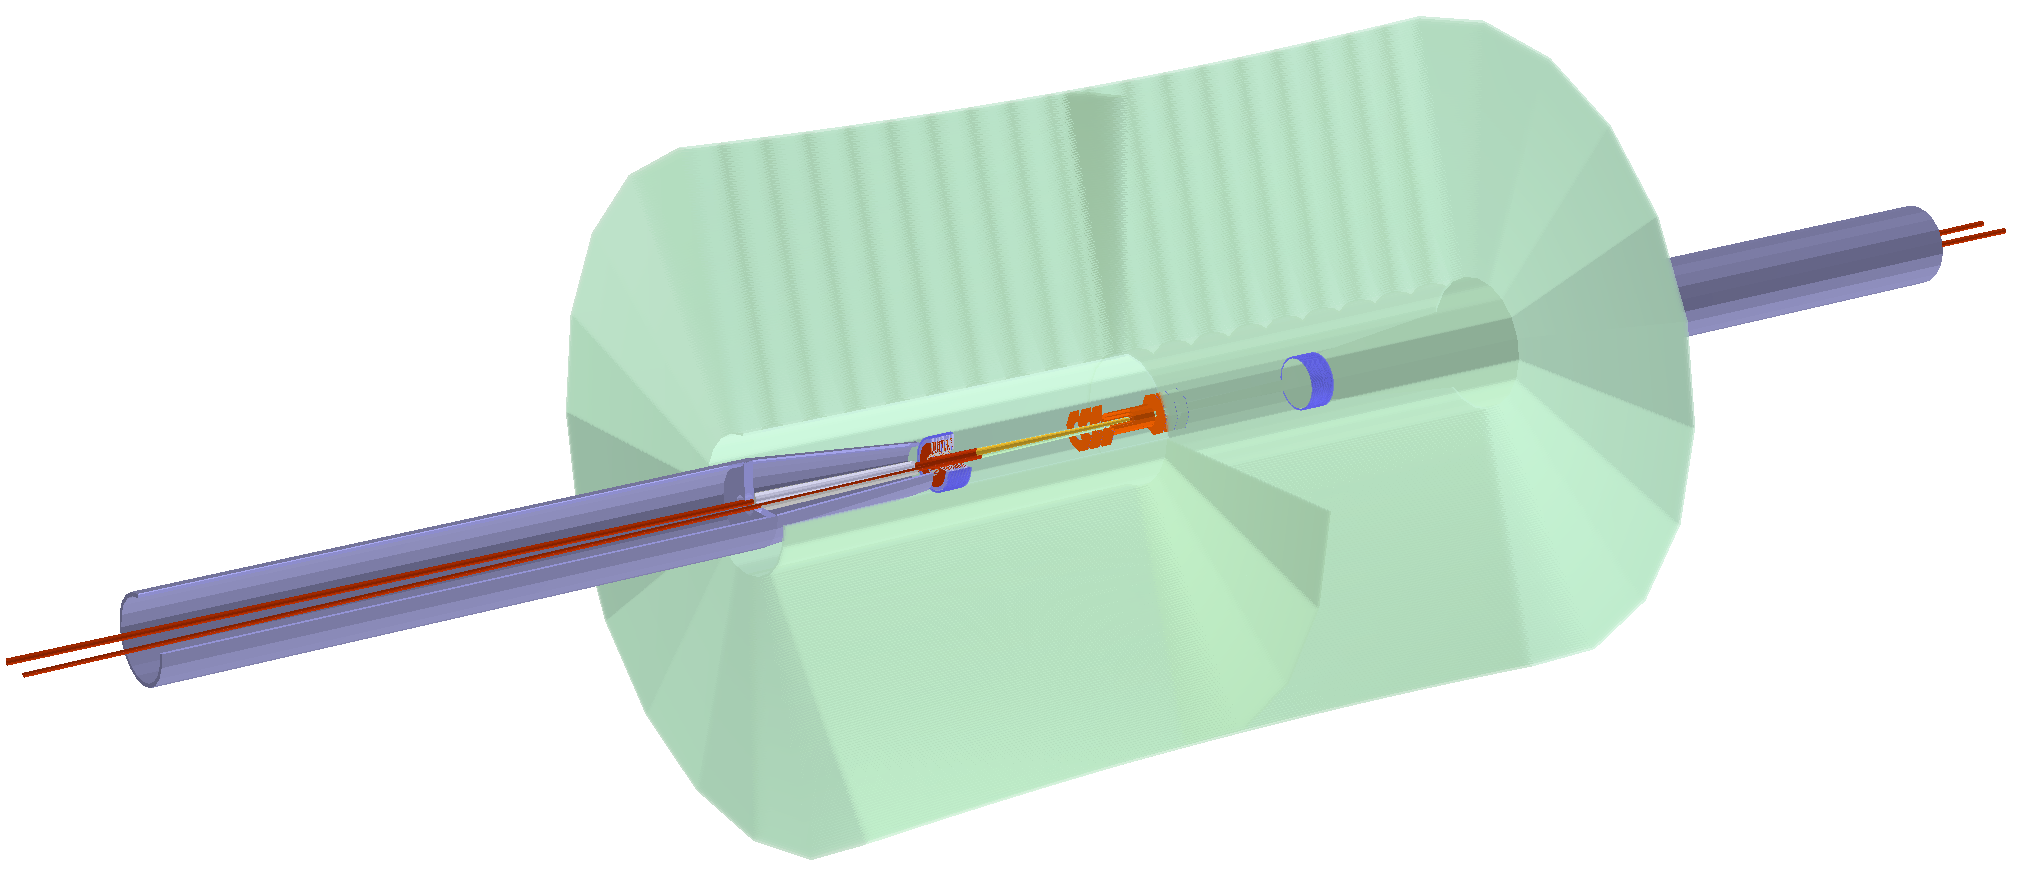
\includegraphics[width=2.5in]{figures/FCCeeIDEA_IR}};
      \begin{scope}[x={(image.south east)},y={(image.north west)}]

%		\draw[help lines,xstep=.1,ystep=.1] (0, 0) grid (1,1);
%        \foreach \x in {0,1,...,9} { \node [anchor=north] at (\x/10,0) {0.\x}; }
%        \foreach \y in {0,1,...,9} { \node [anchor=east] at (0,\y/10)
%         {0.\y}; }
%
        \draw[->, thick](0.2, 0.7) -- (0.4, 0.7);
		\node[left] at (0.2, 0.7) {Drift chamber};

		\draw[->, thick](-0.1, 0.25) -- (0., 0.25);
		\node[left] at (-0.1, 0.25) {Beam pipe};

		\draw[->, thick](0.1, 0.4) -- (0.2, 0.4);
		\node[left] at (0.1, 0.4) {Solenoid shielding};

		\draw[->, thick](0.6, 0.05) -- (0.48, 0.4);
		\node[below] at (0.6, 0.05) {Luminosity calorimeter};

		\draw[->, thick](0.8, 0.2) -- (0.58, 0.5);
		\node[below] at (0.8, 0.2) {Vertex detector};

	\end{scope}
    \end{tikzpicture}
\caption{The detectors at the interaction region for the FCC-ee IDEA concept.}
\label{fig_sim}
\end{figure}

\subsection{Segmentation}

The segmentation of the sensitive gas detector contains the information on the positions of the wires in the detector. The segmentation for the first layer of the drift chamber is shown in \cref{fig_segmentation_first_case}. The total number of wires as a function of the polar angle $\theta$ is illustrated in \cref{fig_segmentation_second_case}.

\begin{figure}[!t]
\centering
\subfloat[]{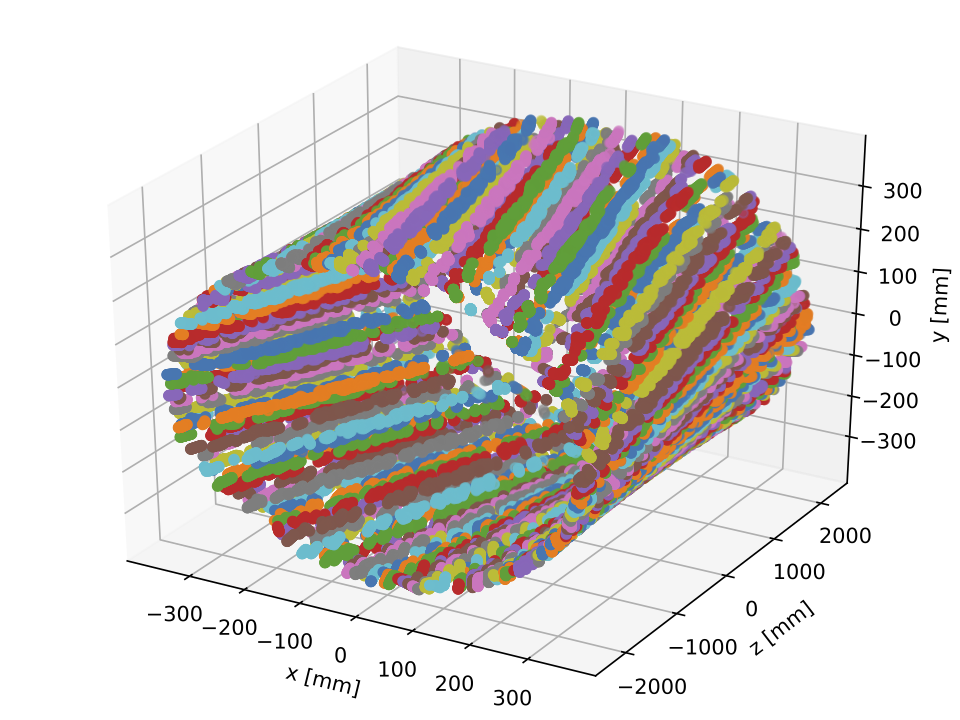
\includegraphics[width=1.5in]{figures/allHits}%
\label{fig_segmentation_first_case}}
\hfil
\subfloat[]{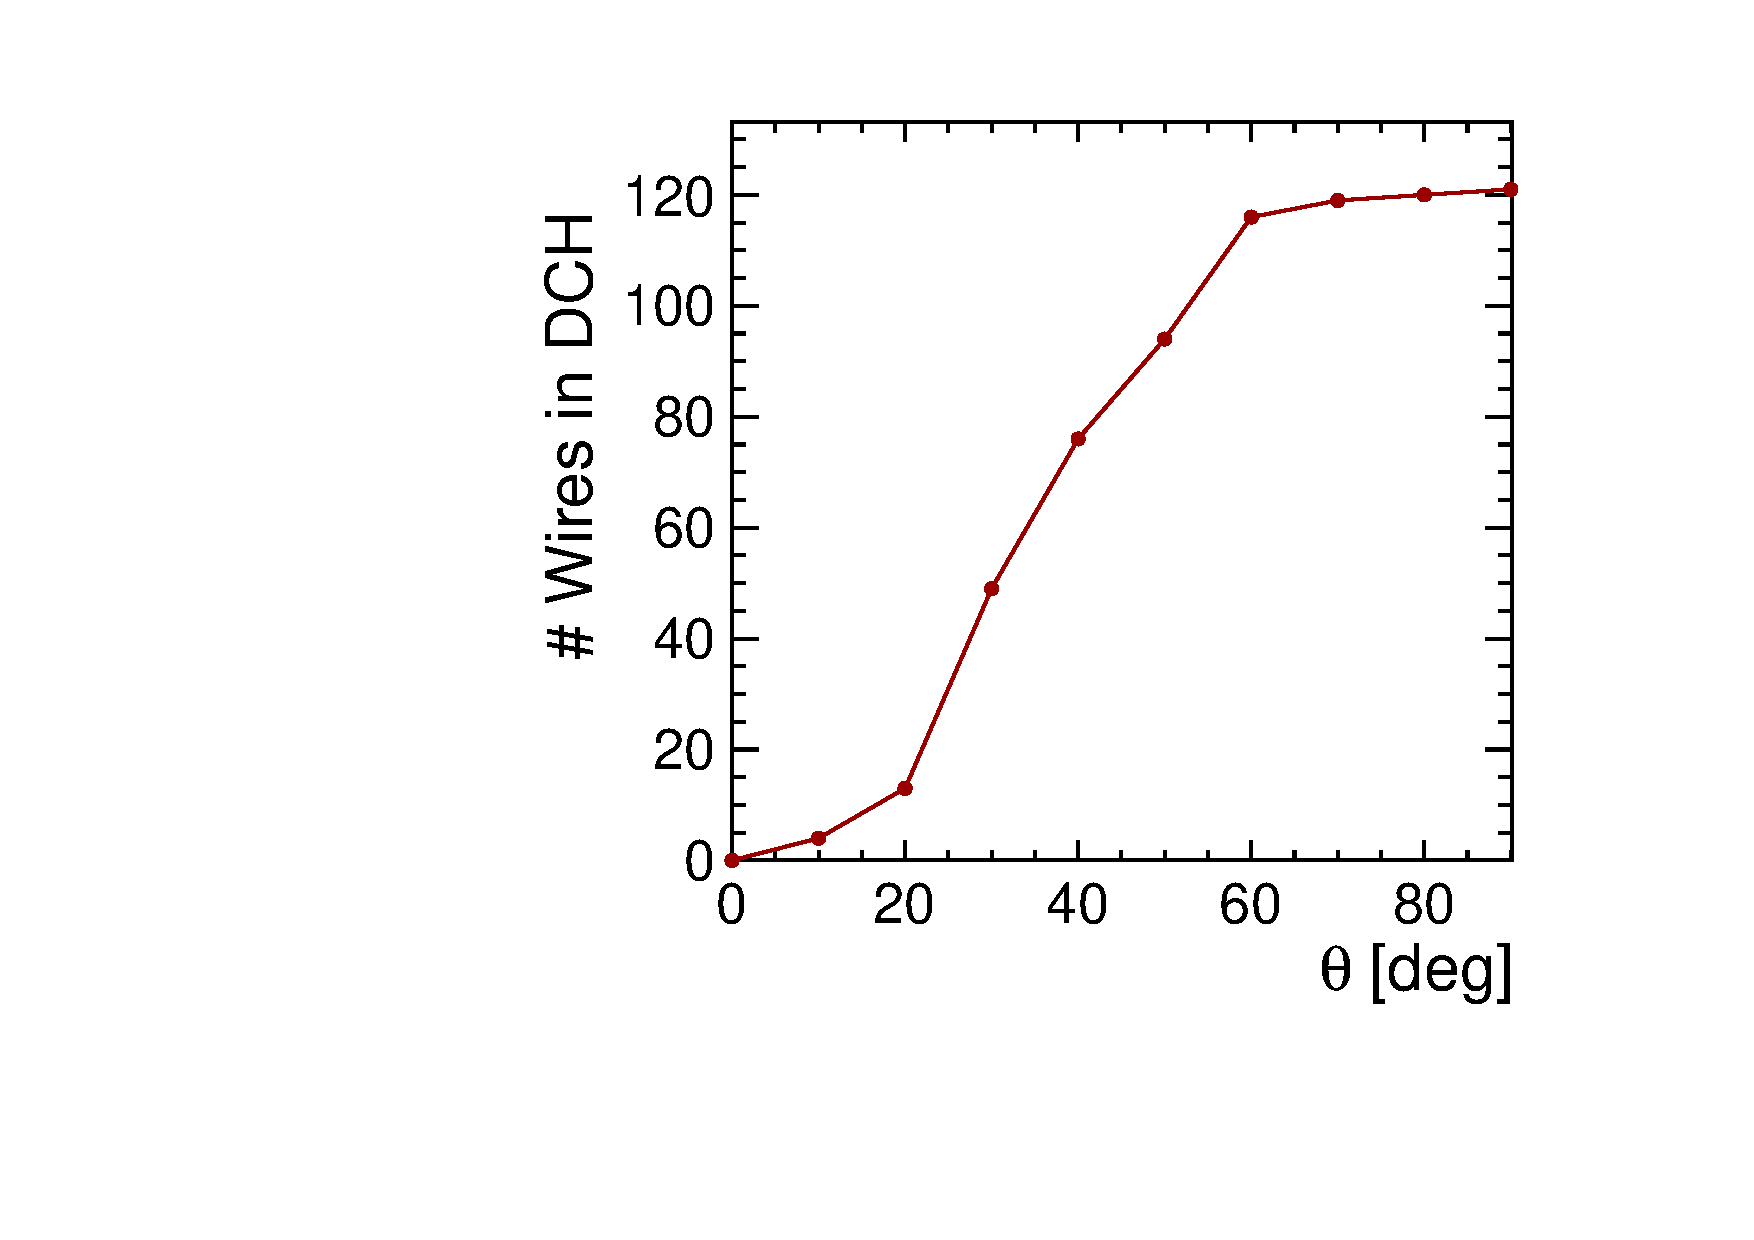
\includegraphics[width=1.5in]{figures/theta_nbHits_DCH}%
\label{fig_segmentation_second_case}}
\caption{(a) shows the segmentation of the first layer of the drift chamber. (b) shows the total number of wires as a function of the polar angle $\theta$.}
\label{fig_segmentation}
\end{figure}


\subsection{\textsc{Geant4} simulation and digitization}
\textsc{Geant4} simulates the passage of particles through matter. For the drift chamber simulation, a step size of 2~mm is chosen in order to step trough the gas volume and calculate the energy deposited. The ionization charge is then drifted to the nearest wire. This allows for calculating the drift time and therefore the signal in the wires. Once the contribution from each \textsc{Geant4} step is calculated, the digitization step regroups the energy deposited with a drift time smaller than the maximum drift time in the cell.

\section{Impact of beam-induced backgrounds}
One of the main sources of background at the FCC-ee experiments is generated from the strong electromagnetic force from the electron and positron bunches in the field of the opposite beam. This leads to the production of Beamstrahlung photons. The interactions of Beamstrahlung photons generate incoherent lepton pairs at low polar angles and mostly contained in the forward direction as shown in~\cref{fig_pairbcg}. The \textsc{GUINEA-PIG}~\cite{Schulte:382453} event generator has been used to generate the incoherent $e^+e^-$ background particles at a $\sqrt{s}$ of $365\,\gev$~\cite{Voutsinas:2017eca} and their impact on the drift chamber is studied below.


\begin{figure}[!t]
\centering
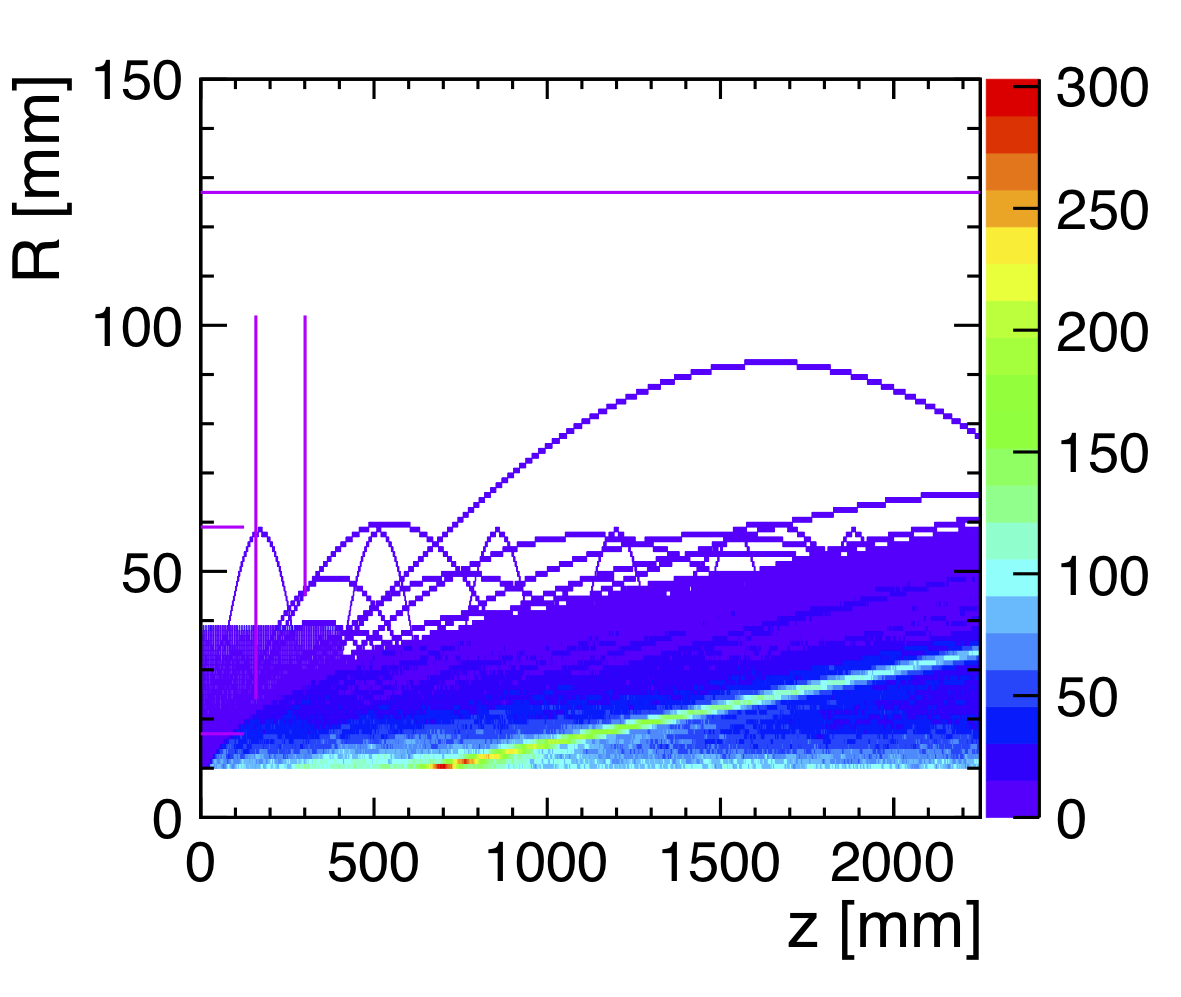
\includegraphics[width=2.5in]{figures/pairs_R_Z.png}
\caption{The trajectory of the $e^+e^-$ pairs in a 2~T magnetic field.}
\label{fig_pairbcg}
\end{figure}

The occupancy due to $e^+e^-$ incoherent pairs in the drift chamber is estimated to $\sim2.85\%$ (averaged over 100 bunch crossings). In fact, the produced incoherent pairs have a low polar angle and only few of them reach the drift chamber. Most of the hits observed are due to the scattering of the pairs by interacting with the elements in the interaction region.

% \begin{figure}[!t]
% \centering
% 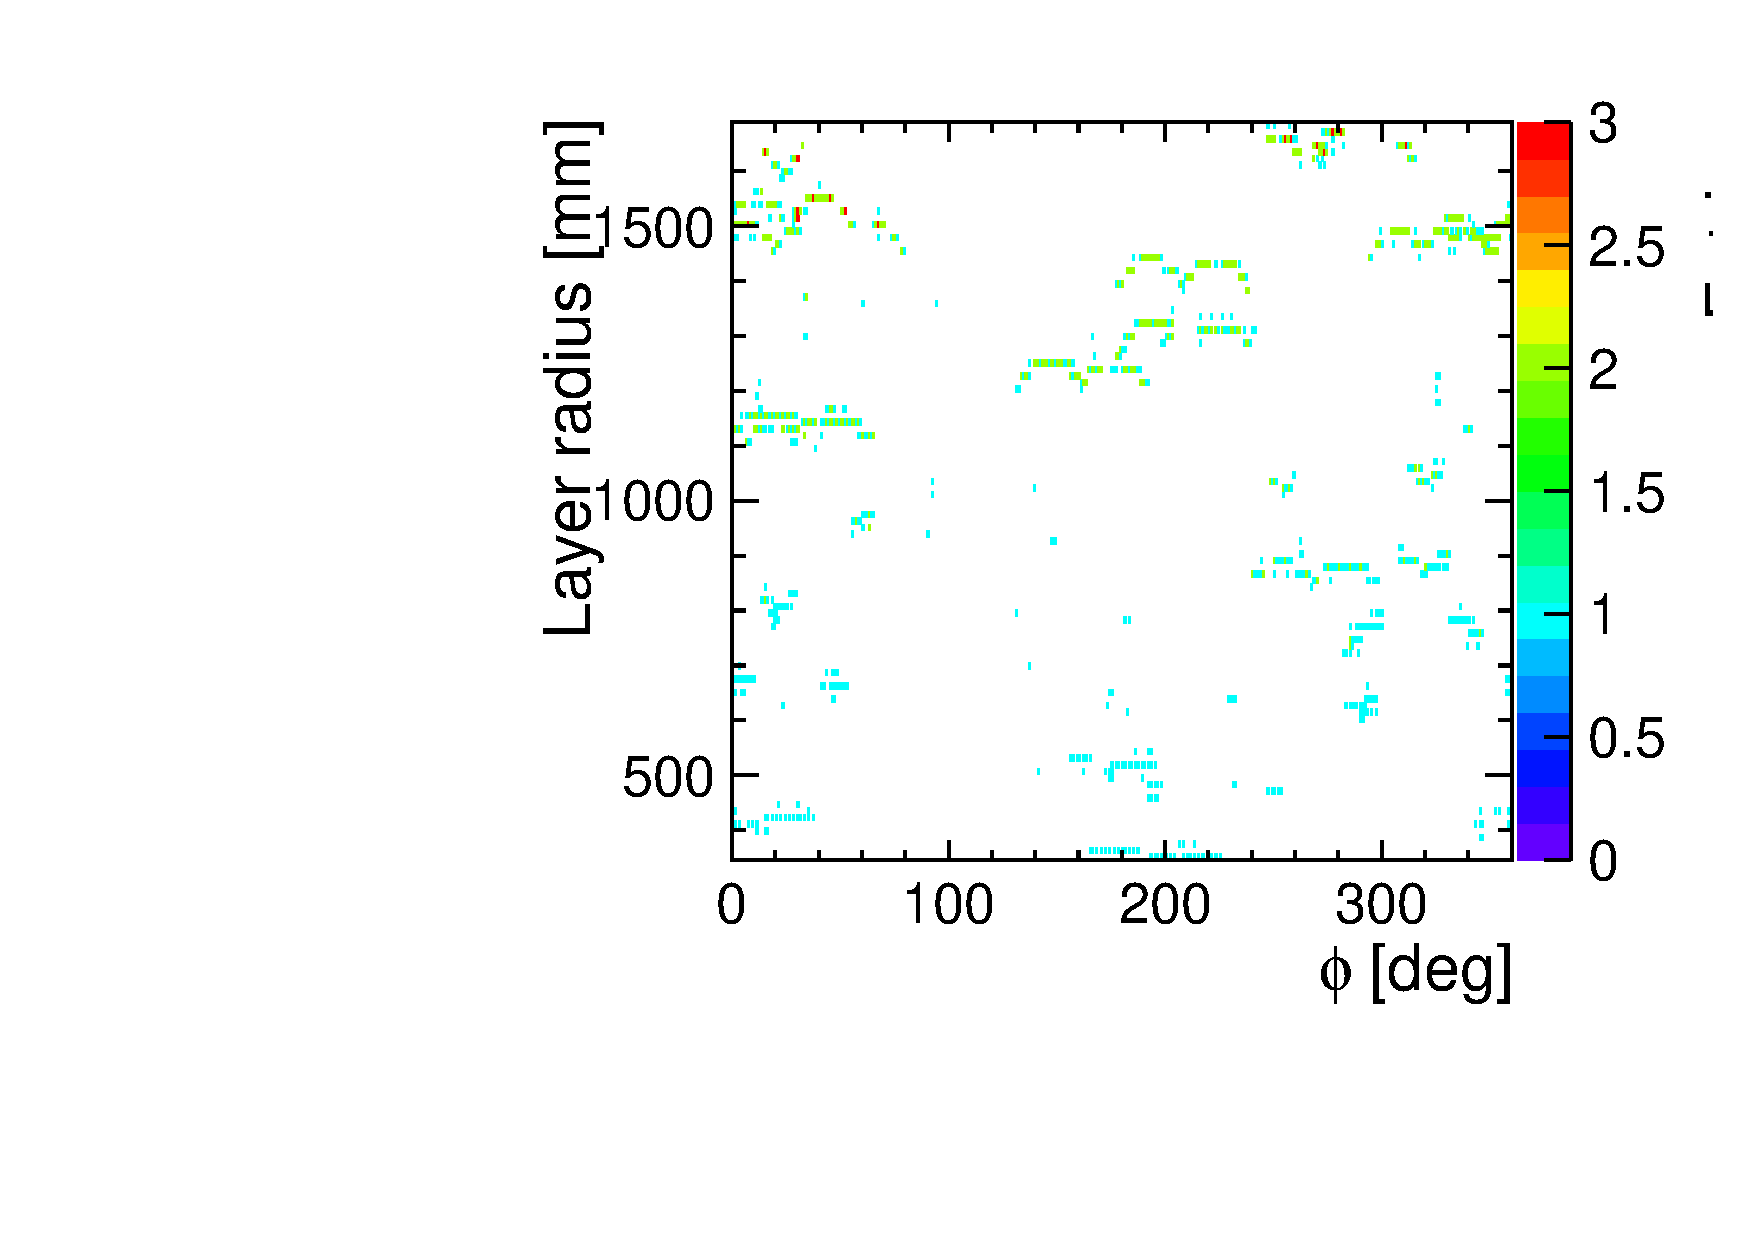
\includegraphics[width=2.5in]{figures/layerR_vs_phi}
% \caption{The detectors at the interaction region for the FCC-ee IDEA concept.}
% \label{fig_simhits}
% \end{figure}

The occupancy of the drift chamber as a function of its radius is shown in~\cref{fig_simhitspercent}. The overall occupancy due to this background remains low and does not pose problems for the reconstruction of the tracks using the drift chamber.

\begin{figure}[!t]
\centering
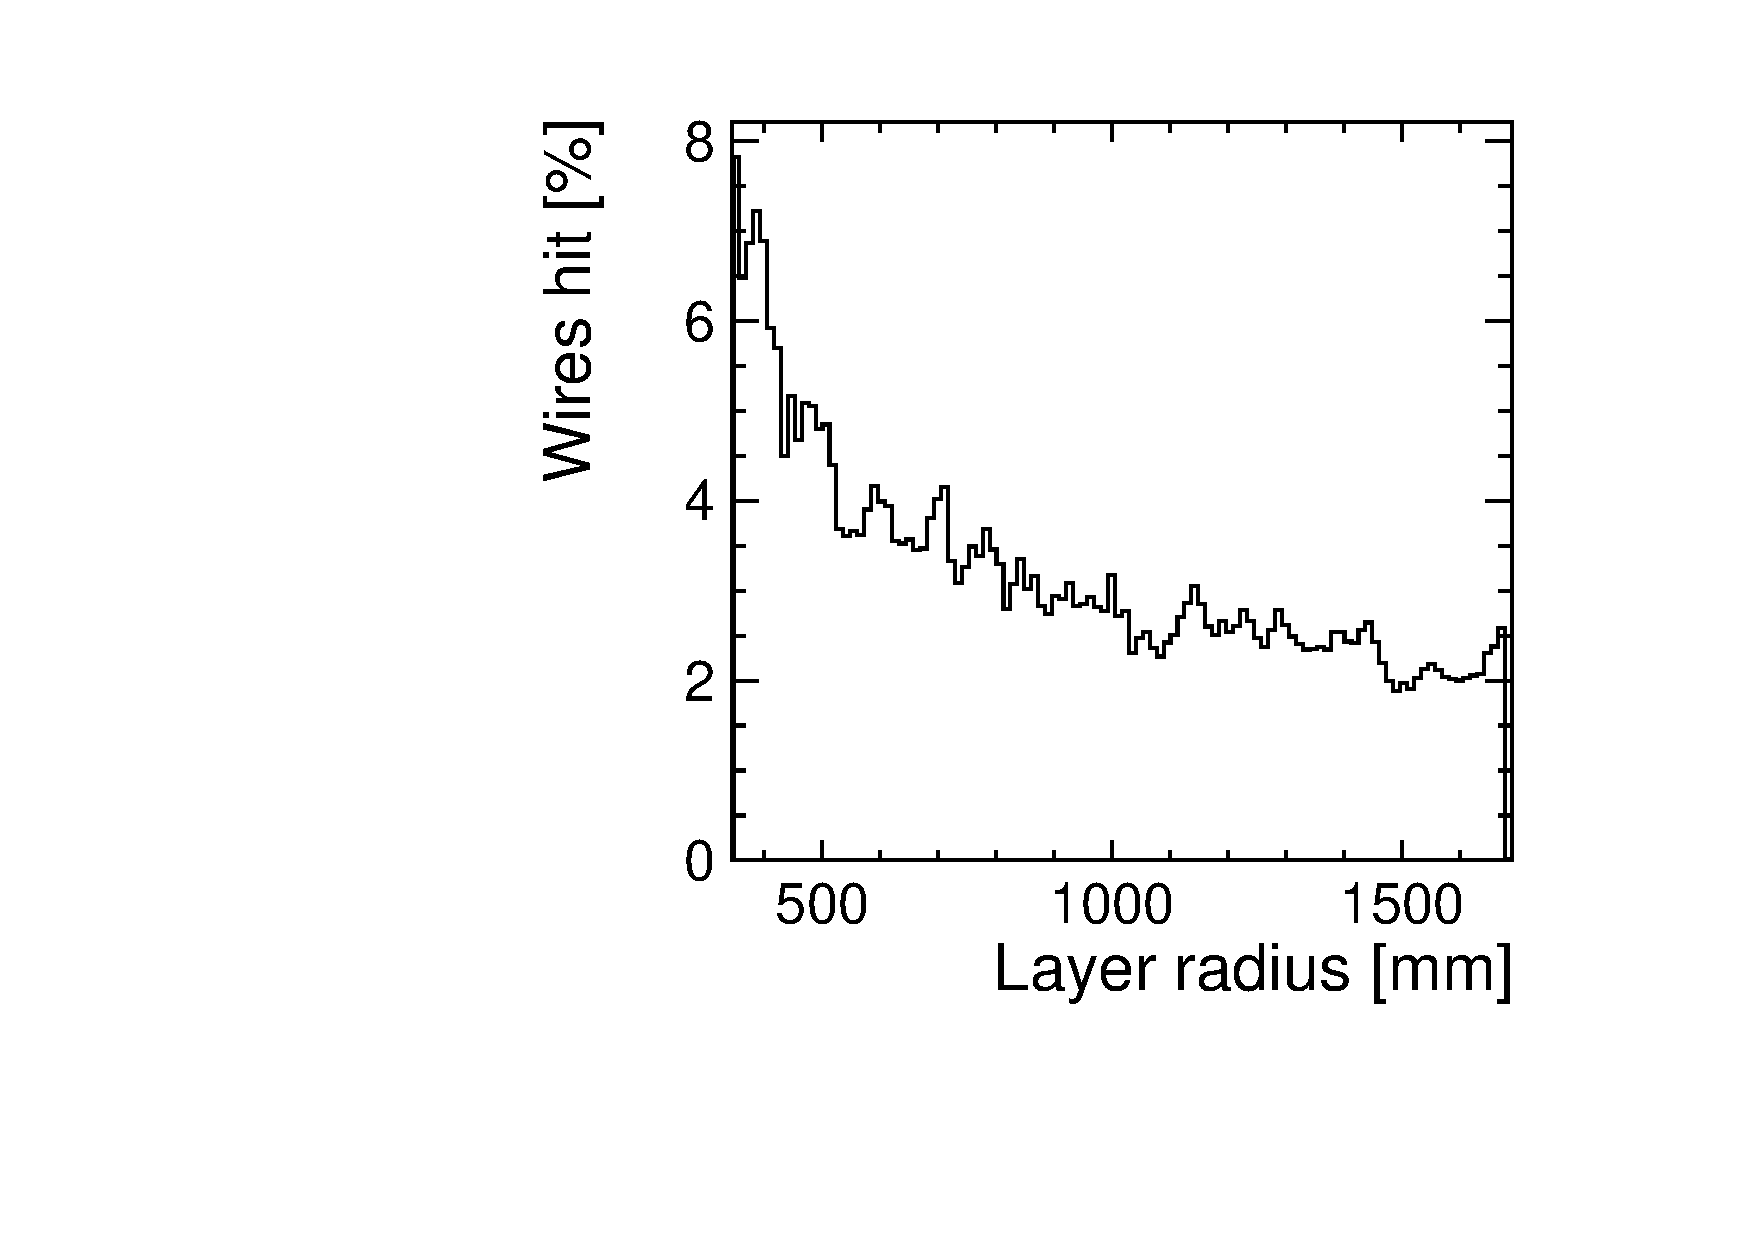
\includegraphics[width=2.5in]{figures/layerR_vs_wires_percent}
\caption{The percentage of wires hit due to $e^+e^-$ background as a function of the layer radius averaged over 100 bunch crossings.}
\label{fig_simhitspercent}
\end{figure}

\section{Conclusion}
The drift chamber for the IDEA detector concept has been investigated in full simulations using the FCCSW. The full simulation chain has been implemented and validated using this common software and the impact of one of the most important beam-induced backgrounds due to the incoherent $e^+e^-$ pairs has been investigated in simulations. The overall impact remains low and does not pose problems for the track reconstruction with this detector.


% use section* for acknowledgment
% \section*{Acknowledgment}
%
% The authors would like to thank...



% Note that the IEEE typically puts floats only at the top, even when this
% results in a large percentage of a column being occupied by floats.


% An example of a double column floating figure using two subfigures.
% (The subfig.sty package must be loaded for this to work.)
% The subfigure \label commands are set within each subfloat command,
% and the \label for the overall figure must come after \caption.
% \hfil is used as a separator to get equal spacing.
% Watch out that the combined width of all the subfigures on a
% line do not exceed the text width or a line break will occur.
%
%\begin{figure*}[!t]
%\centering
%\subfloat[Case I]{\includegraphics[width=2.5in]{box}%
%\label{fig_first_case}}
%\hfil
%\subfloat[Case II]{\includegraphics[width=2.5in]{box}%
%\label{fig_second_case}}
%\caption{Simulation results for the network.}
%\label{fig_sim}
%\end{figure*}
%
% Note that often IEEE papers with subfigures do not employ subfigure
% captions (using the optional argument to \subfloat[]), but instead will
% reference/describe all of them (a), (b), etc., within the main caption.
% Be aware that for subfig.sty to generate the (a), (b), etc., subfigure
% labels, the optional argument to \subfloat must be present. If a
% subcaption is not desired, just leave its contents blank,
% e.g., \subfloat[].


% An example of a floating table. Note that, for IEEE style tables, the
% \caption command should come BEFORE the table and, given that table
% captions serve much like titles, are usually capitalized except for words
% such as a, an, and, as, at, but, by, for, in, nor, of, on, or, the, to
% and up, which are usually not capitalized unless they are the first or
% last word of the caption. Table text will default to \footnotesize as
% the IEEE normally uses this smaller font for tables.
% The \label must come after \caption as always.
%
%\begin{table}[!t]
%% increase table row spacing, adjust to taste
%\renewcommand{\arraystretch}{1.3}
% if using array.sty, it might be a good idea to tweak the value of
% \extrarowheight as needed to properly center the text within the cells
%\caption{An Example of a Table}
%\label{table_example}
%\centering
%% Some packages, such as MDW tools, offer better commands for making tables
%% than the plain LaTeX2e tabular which is used here.
%\begin{tabular}{|c||c|}
%\hline
%One & Two\\
%\hline
%Three & Four\\
%\hline
%\end{tabular}
%\end{table}


% Note that the IEEE does not put floats in the very first column
% - or typically anywhere on the first page for that matter. Also,
% in-text middle ("here") positioning is typically not used, but it
% is allowed and encouraged for Computer Society conferences (but
% not Computer Society journals). Most IEEE journals/conferences use
% top floats exclusively.
% Note that, LaTeX2e, unlike IEEE journals/conferences, places
% footnotes above bottom floats. This can be corrected via the
% \fnbelowfloat command of the stfloats package.









% trigger a \newpage just before the given reference
% number - used to balance the columns on the last page
% adjust value as needed - may need to be readjusted if
% the document is modified later
%\IEEEtriggeratref{8}
% The "triggered" command can be changed if desired:
%\IEEEtriggercmd{\enlargethispage{-5in}}

% references section

% can use a bibliography generated by BibTeX as a .bbl file
% BibTeX documentation can be easily obtained at:
% http://mirror.ctan.org/biblio/bibtex/contrib/doc/
% The IEEEtran BibTeX style support page is at:
% http://www.michaelshell.org/tex/ieeetran/bibtex/
\bibliographystyle{IEEEtran}
% argument is your BibTeX string definitions and bibliography database(s)
\bibliography{ref.bib}
%
% <OR> manually copy in the resultant .bbl file
% set second argument of \begin to the number of references
% (used to reserve space for the reference number labels box)



%\begin{thebibliography}{1}

%\bibitem{IEEEhowto:kopka}
%H.~Kopka and P.~W. Daly, \emph{A Guide to \LaTeX}, 3rd~ed.\hskip 1em plus
%  0.5em minus 0.4em\relax Harlow, England: Addison-Wesley, 1999.
%
%\end{thebibliography}




% that's all folks
\end{document}
